%%%%%%%%%%%%%%%%%%%%%%%%%%%%%%%%%
%
%       EXERCÍCIO
%
%%%%%%%%%%%%%%%%%%%%%%%%%%%%%%%%%

\definevalorquestao

\begin{exercicioBanco}[\valorquestao]
Em um laboratório de química, a temperatura $T(t)$ (em $^{\circ}\text{C}$) de uma reação controlada é monitorada em função do tempo $t$ (em horas) através da função exponencial da forma $T(t) = a \cdot 3^t + b$, onde $a$ e $b$ são constantes reais. 

O gráfico a seguir descreve a evolução da temperatura ao longo do tempo, destacando a temperatura inicial no instante $t = 0$ e a temperatura após $2$ horas.

\begin{center}
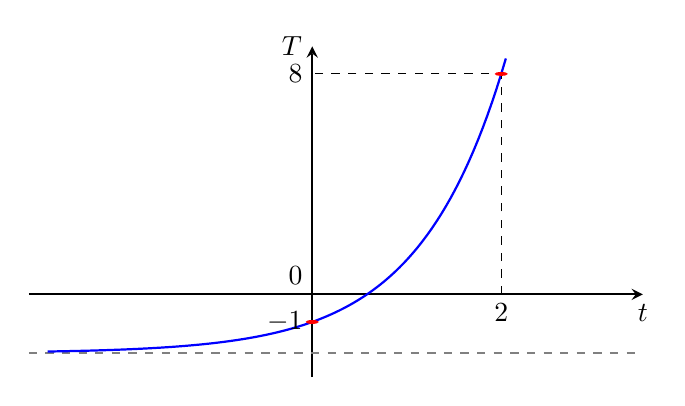
\begin{tikzpicture}[xscale=1.2, yscale=0.35, >=stealth]
    % Eixos cartesiano
    \draw[->, thick] (-3,0) -- (3.5,0) node[below] {$t$};
    \draw[->, thick] (0,-3) -- (0,9) node[left] {$T$};
    \node[above left] at (0,0) {$0$};
    
    % Assíntota horizontal
    \draw[dashed, gray] (-3,-2.125) -- (3.5,-2.125);
    
    % Gráfico da função f(t) = (9/8)*3^t - 17/8
    \draw[thick, blue, domain=-2.8:2.05, samples=100] plot (\x, {1.125*3^(\x) - 2.125});
    
    % Marcadores dos pontos (0, -1) e (2, 8)
    \draw[dashed] (2,0) -- (2,8) -- (0,8);
    \node[below] at (2,0) {$2$};
    \node[left] at (0,8) {$8$};
    \node[left] at (0,-1) {$-1$};
    
    \fill[red] (0,-1) circle (2pt);
    \fill[red] (2,8) circle (2pt);
\end{tikzpicture}
\end{center}

Nessas condições, o valor aproximado da temperatura estabilizada dessa reação após um longo período de tempo (limite inferior dado pela assíntota do gráfico) é obtido pelo valor da constante $b$. Pode-se dizer que o valor exato de $b$ é igual a:

\newcommand{\alternativas}{%
    \begin{center}
        \begin{tabularx}{\textwidth}{XXXXX}
            (a) \(-\dfrac{17}{8}\). &
            (b) \(-\dfrac{9}{8}\). &
            (c) \(-1\). &
            (d) \(-\dfrac{5}{2}\). &
            (e) \(-\dfrac{15}{8}\).
        \end{tabularx}
    \end{center}
}

\newcommand{\resposta}{A}

% Lógica condicional para exibição
\ifdefstring{\atividade}{lista}{%
    \alternativas
    \vspace{0.5em}
    
    \noindent\textbf{Resposta:} letra \textbf{\resposta}.
}{%
    \ifdefstring{\modo}{objetivo}{%
        \alternativas
    }{%
        % modo = discursiva → não mostra alternativas
    }
}
\end{exercicioBanco}

